\documentclass{beamer}
\usepackage{amsmath}
\usepackage[english]{babel} %set language; note: after changing this, you need to delete all auxiliary files to recompile
\usepackage[utf8]{inputenc} %define file encoding; latin1 is the other often used option
\usepackage{csquotes} % provides context sensitive quotation facilities
\usepackage{graphicx} %allows for inserting figures
\usepackage{booktabs} % for table formatting without vertical lines
\usepackage{textcomp} % allow for example using the Euro sign with \texteuro
\usepackage{stackengine}
\usepackage{wasysym}
\usepackage{tikzsymbols}
\usepackage{textcomp}
\usepackage{ragged2e} 
\usepackage{graphicx}  
\usepackage{tikz}  
% ELIMINAR COMANDOS DE NAVEGACION%%%%%%%%%%%
\setbeamertemplate{navigation symbols}

%\newcommand{\bubblethis}[2]{
 %       \tikz[remember picture,baseline]{\node[anchor=base,inner sep=0,outer sep=0]%
 %       (#1) {\underline{#1}};\node[overlay,cloud callout,callout relative pointer={(0.2cm,-0.7cm)},%
 %       aspect=2.5,fill=yellow!90] at ($(#1.north)+(-0.5cm,1.6cm)$) {#2};}%
 %   }%
%\tikzset{face/.style={shape=circle,minimum size=4ex,shading=radial,outer sep=0pt,
 %       inner color=white!50!yellow,outer color= yellow!70!orange}}

%% Some commands to make the code easier
\newcommand{\emoticon}[1][]{%
  \node[face,#1] (emoticon) {};
  %% The eyes are fixed.
  \draw[fill=white] (-1ex,0ex) ..controls (-0.5ex,0.2ex)and(0.5ex,0.2ex)..
        (1ex,0.0ex) ..controls ( 1.5ex,1.5ex)and( 0.2ex,1.7ex)..
        (0ex,0.4ex) ..controls (-0.2ex,1.7ex)and(-1.5ex,1.5ex)..
        (-1ex,0ex)--cycle;}
\newcommand{\pupils}{
  %% standard pupils
  \fill[shift={(0.5ex,0.5ex)},rotate=80] 
       (0,0) ellipse (0.3ex and 0.15ex);
  \fill[shift={(-0.5ex,0.5ex)},rotate=100] 
       (0,0) ellipse (0.3ex and 0.15ex);}

\newcommand{\emoticonname}[1]{
  \node[below=1ex of emoticon,font=\footnotesize,
        minimum width=4cm]{#1};}
\usepackage{scalerel}
\usetikzlibrary{positioning}
\usepackage{xcolor,amssymb}
\newcommand\dangersignb[1][2ex]{%
  \scaleto{\stackengine{0.3pt}{\scalebox{1.1}[.9]{%
  \color{red}$\blacktriangle$}}{\tiny\bfseries !}{O}{c}{F}{F}{L}}{#1}%
}
\newcommand\dangersignw[1][2ex]{%
  \scaleto{\stackengine{0.3pt}{\scalebox{1.1}[.9]{%
  \color{red}$\blacktriangle$}}{\color{white}\tiny\bfseries !}{O}{c}{F}{F}{L}}{#1}%
}
\usepackage{fontawesome} % Social Icons
\usepackage{epstopdf} % allow embedding eps-figures
\usepackage{tikz} % allows drawing figures
\usepackage{amsmath,amssymb,amsthm} %advanced math facilities
\usepackage{lmodern} %uses font that support italic and bold at the same time
\usepackage{tikz}
\hypersetup{
    colorlinks=true,
    linkcolor=blue,
    filecolor=magenta,      
    urlcolor=blue,
}
\usepackage{tcolorbox}
\usepackage{hyperref}

\usefonttheme[onlymath]{serif} %set math font to serif ones

\definecolor{beamerblue}{rgb}{0.2,0.2,0.7} %define beamerblue color for later use

%%% defines highlight command to set text blue
\newcommand{\highlight}[1]{{\color{blue}{#1}}}


%%%%%%% commands defining backup slides so that frame numbering is correct

\newcommand{\backupbegin}{
   \newcounter{framenumberappendix}
   \setcounter{framenumberappendix}{\value{framenumber}}
}
\newcommand{\backupend}{
   \addtocounter{framenumberappendix}{-\value{framenumber}}
   \addtocounter{framenumber}{\value{framenumberappendix}}
}

%%%% end of defining backup slides

%Specify figure caption, see also http://tex.stackexchange.com/questions/155738/caption-package-not-working-with-beamer
\setbeamertemplate{caption}{\insertcaption} %redefines caption to remove label "Figure".
%\setbeamerfont{caption}{size=\scriptsize,shape=\itshape,series=\bfseries} %sets figure  caption bold and italic and makes it smaller


\usetheme{Boadilla}

%set options of hyperref package
\hypersetup{
    bookmarksnumbered=true, %put section numbers in bookmarks
    naturalnames=true, %use LATEX-computed names for links
    citebordercolor={1 1 1}, %color of border around cites, here: white, i.e. invisible
    linkbordercolor={1 1 1}, %color of border around links, here: white, i.e. invisible
    colorlinks=true, %color links
    anchorcolor=black, %set color of anchors
    linkcolor=beamerblue, %set link color to beamer blue
    citecolor=blue, %set cite color to beamer blue
    pdfpagemode=UseThumbs, %set default mode of PDF display
    breaklinks=true, %break long links
    pdfstartpage=1 %start at first page
    }

\newtcolorbox{boxA}{
    fontupper = \bf,
    boxrule = 1.5pt,
    colframe = black % frame color
}

\newtcolorbox{boxB}{
    boxrule = 1.5pt,
    colframe = blue!70!black,, % frame color
    colback = blue!7!white,
}

% --------------------
% Overall information
% --------------------
\title[Principios de Economía]{Principios de Economía \vspace{4mm}
\\ Magistral 2}
\date{}
\author[Franco Riottini]{Franco Riottini}
\vspace{0.4cm}
\institute[]{Universidad de San Andrés} 

\begin{document}

\begin{frame}
\titlepage
\centering
\includegraphics[scale=0.2]{../Figures/logoUDESA.jpg} 
\end{frame}


\begin{frame}
\frametitle{La economía, los modelos y las funciones}
\begin{itemize}
    \item La economía estudia cómo asignar recursos escasos de forma eficiente
    \item Las funciones (y sus expresiones matemáticas y gráficas) nos ayudan a representar ideas...
    \item Vamos a utilizar funciones para crear un modelo que nos permita analizar como los individuos manejan la ESCASEZ 
    \begin{itemize}
        \item ¿Qué significa que los recursos son escasos? ¡Que no hay de todo para todos!
    \end{itemize}
    \item El problema surge porque las necesidades humanas son, en la práctica, ilimitadas, mientras que los recursos económicos son limitados. 
    \begin{boxA}
        \begin{center}
        
            La escasez representa básicamente una restricción o límite que nos obliga a elegir entre alternativas.
        
        \end{center}
    \end{boxA} 
\end{itemize} 
\end{frame}

\begin{frame}{Trade-off}
    \begin{itemize}
        \item Cada vez que tomamos una decisión y elegimos algo, ganamos algo pero también perdemos algo \vspace{2mm}
        \item ¿Cómo tomamos una decisión? 
        \begin{itemize}
            \item Evaluamos todos los \textbf{beneficios} que se obtienen por tomar la decisión y compararlos con todos los \textbf{costos} que resultan de la decisión
            \vspace{1mm}
        \end{itemize}
        \item A veces es fácil pensar en esto, pero otras veces no tanto...
        \item ¿Cómo podemos cuantificar los beneficios y los costos?
    \end{itemize} 
\end{frame}

\begin{frame}{Beneficios y costos}
    \begin{itemize}
        \item \textbf{Beneficios}: Lo que se \textbf{gana} por realizar una actividad
        \begin{itemize}
            \item Puede ser monetario si está evaluado en el mercado
            \item Pero tambien puede no ser monetario (tiempo, salud, \textbf{bienestar, utilidad}, etc.)
        \end{itemize}
        \item \textbf{Costos}: Todos los recursos que \textbf{resigno} para llevar a cabo una actividad.
    \end{itemize} 
\end{frame}

\begin{frame}{¿Cuáles son los costos relevantes? }
    \begin{itemize}
        \item \textcolor{blue}{Costos dependientes de la actividad}
        \item \href{https://econ.video/2017/08/28/the-simpsons-opportunity-cost-of-lines/}{Costo de oportunidad}
        \begin{itemize}
        \vspace{2mm}
            \item  El costo de oportunidad de una decisión es el valor al que se renuncia al rechazar la mejor alternativa posible.
        \end{itemize}
        \vspace{2mm}
        \item \textcolor{red}{Costo hundido}
        \begin{itemize}
        \vspace{2mm}
        \item Costos en los que ya se ha incurrido y no se pueden recuperar.
        \end{itemize}
        \vspace{2mm}
        \begin{itemize}
        \item \textbf{La falacia del costo hundido.}  
            \begin{itemize}
            \item Ocurre cuando se están considerando costos y beneficios que no varían con las consecuencias de su decisión
            \item  "Regla": si tengo que afrontar un costo sea cual sea la decisión que tome, entonces es un costo hundido y no lo debo tener en cuenta!
            \end{itemize}
        \end{itemize}
    \end{itemize} 
\end{frame}

\begin{frame}{Entonces.. }
    \begin{itemize}
        \item ¿Cómo podemos cuantificar los beneficios y los costos? 
        \begin{itemize}
        \item Cuando disponemos de ``precios de mercado'' se facilita la cuestión
        \item Veamos un ejemplo: delivery o cocinar.
        \end{itemize}
        \item La regla para tomar decisiones:
        \begin{boxB}
            \justify{Elegimos una alternativa si y sólo si la \textbf{variación} que experimentarán los beneficios como consecuencia de elegir dicha alternativa excede a la variación que experimentarán los costos.} \\ \vspace{2mm}
            \textbf{Beneficios marginales vs costos marginales} \centering 
        \end{boxB}
    \end{itemize} 
\end{frame}
\begin{frame}
\frametitle{Pensemos algunos casos}
\begin{itemize}
    \item Vamos a usar los conceptos y el modelo para comprender como las personas toman decisiones: \vspace{2mm}
    \begin{itemize} 
    \item ¿Que sucede si \textbf{pierdo} la entrada que compre para el recital de Taylor Swift? \vspace{2mm}
    \item ¿Por qué solo en las grandes ciudades los Remis/Taxis están pintados de un mismo color? \vspace{2mm}
    \item ¿Por qué los colectivos escolares no tienen cinturón de seguridad? 
    \end{itemize}
\end{itemize} 
\end{frame}

\begin{frame}{¿Tik tok es gratis?}
    \begin{itemize}
        \item Los Argentinos pasamos en promedio 30 minutos diarios en Tik Tok. \vspace{2mm}
        \item En jóvenes el tiempo puede superar las dos horas diarias. \vspace{2mm}
        \begin{itemize}
        \item ¿Cuál es el costo de oportunidad por hora? \vspace{2mm}
        \item Estimemos el costo de oportunidad total... \\ \pause \vspace{2mm}
        Si una persona podría ganar \$4.000 por hora trabajando y pasa 2 horas diarias en TikTok, \vspace{2mm} \pause 
        \begin{itemize}
         \item Costo de oportunidad diario: \$8.000. 
         \item Costo de oportunidad mensual: \$160.000. 
         \item Costo de oportunidad anual: \$1.920.000. 
        \end{itemize}
        \vspace{2mm} \pause 
        \item ¿Para Messi es igual?
        \end{itemize}
    \end{itemize} 
\end{frame}

\begin{frame}{La decisión de consumo}
    \begin{itemize}
    \item ¿Qué tiene en cuenta un consumidor al momento de consumir un producto? \vspace{2mm}
    \item ¿Qué información necesitamos? \vspace{2mm}
    \begin{itemize}
        \item Ingreso/dinero disponible \vspace{2mm}
        \item Precios de todos los productos \vspace{2mm}
        \item Preferencias o gustos
        \end{itemize}
    \end{itemize}
\end{frame}

\begin{frame}{El problema del estudiante}
    \begin{center}
    \begin{tikzpicture}
        % Ejes
        \draw[thick,->] (0,0) -- (6,0) node[below] {Pizza};
        \draw[thick,->] (0,0) -- (0,5.5) node[left] {Cerveza};
    
        % Imágenes
        \node at (0.7,4.5) {\includegraphics[width=1.2cm]{../Figures/cerveza.png}};
        \node at (5,0.8) {\includegraphics[width=1.5cm]{../Figures/pizza.jpg}};
    
        % Texto
        \node at (5,5) {\textbf{{\large ¡NOCHE DE FIESTA!}}};
        \node at (5,4.5) {\textbf{{Tiene \$2000 para gastar}}};
    
        % Etiquetas de precios
        \node[left] at (-0.5,4) {1 cerveza a \$100};
        \node[below] at (4,-0.6) {1 porción de pizza a \$50};
    
        % Flechas y descripciones
        \draw[->] (-0.5,4) -- (-0.1,4.5);
        \draw[->] (4.7,-0.5) -- (5,-0.1);
    \end{tikzpicture}
    \end{center}
\end{frame}
    
\begin{frame}{¿Cómo construimos la restricción presupuestaria?} 
    \begin{center}
    \begin{tikzpicture}
        % Ejes
        \draw[thick,->] (0,0) -- (5,0) node[below] {Pizza};
        \draw[thick,->] (0,0) -- (0,5) node[left] {Cerveza};
    
        % Texto y flecha 1 (Aparece en la segunda diapositiva)
        \only<2->{
            \fill (0,4) circle (2pt) node[left] {20};
            \draw[->] (-0.1,3.8) -- (-0.5,3.4);
            \node[left] at (-0.5,3.5) {Todo el dinero se};
            \node[left] at (-0.6,3.1) {gasta en cerveza};
        }
        % Texto y flecha 3 (Aparece en la tercera diapositiva)
        \only<3->{
            \fill (4,0) circle (2pt) node[below] {40};
            \draw[->] (4.1,0.1) -- (4.5,0.6);
            \node[right] at (4,1.5) {Todo el dinero se};
            \node[right] at (4,1) {gasta en pizza};
        }
        \only<4->{\draw[thick] (0,4) -- (4,0); 
        }
        % Texto y flecha 2 (Aparece en la cuarta diapositiva)
        \only<5->{
            \fill (2,2) circle (2pt) node[above] {A};
            \draw[dashed] (2,2) -- (2,0) node[below] {20};
            \draw[dashed] (2,2) -- (0,2) node[left] {10};
            \draw[->] (2.2,2.1) -- (2.8,2.6);
            \node[right] at (3,3.2) {La mitad se gasta en cervezas};
            \node[right] at (3,2.8) {y la otra mitad en pizzas};
        }
    \end{tikzpicture}
    \end{center}
\end{frame}
    
\begin{frame}{Canastas factibles vs canastas inalcanzables} 
    \begin{center}
    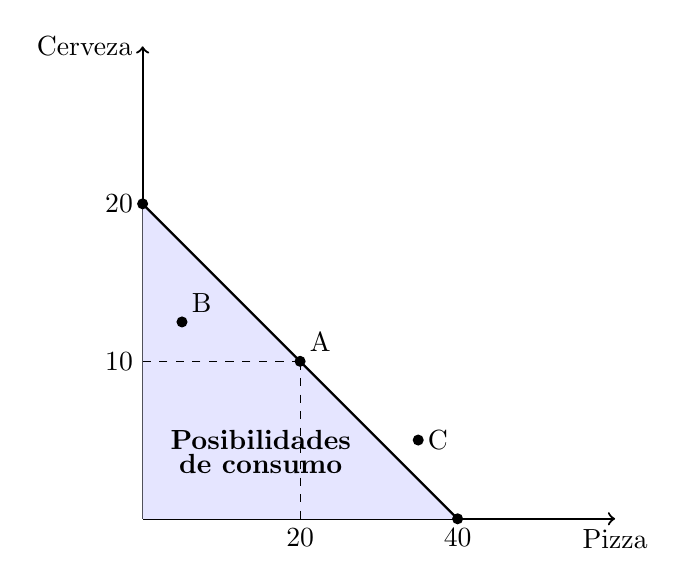
\begin{tikzpicture}
        % Ejes
        \draw[thick,->] (0,0) -- (6,0) node[below] {Pizza};
        \draw[thick,->] (0,0) -- (0,6) node[left] {Cerveza};
    
        % Área sombreada (Posibilidades de consumo)
        \fill[blue!10] (0,4) -- (4,0) -- (0,0) -- cycle;
    
        % RP
        \draw[thick] (0,4) -- (4,0);
    
        % Puntos clave
        \fill (0,4) circle (2pt) node[left] {20};
        \fill (4,0) circle (2pt) node[below] {40};
        \fill (2,2) circle (2pt) node[above right] {A};
        
        % Líneas punteadas
        \draw[dashed] (2,2) -- (2,0) node[below] {20};
        \draw[dashed] (2,2) -- (0,2) node[left] {10};
    
        % Puntos adicionales B y C
        \fill (0.5,2.5) circle (2pt) node[above right] {B};
        \fill (3.5,1) circle (2pt) node[right] {C};
    
        % Texto dentro del área sombreada
        \node at (1.5,1) {\textbf{Posibilidades}};
        \node at (1.5,0.7) {\textbf{de consumo}};
    
    \end{tikzpicture}
    \end{center}
\end{frame}
    
\begin{frame}{Restricción presupuestaria}
    \begin{itemize}
        \item La restricción presupuestaria determina las cantidades de bienes que pueden ser adquiridas por el agente dado el presupuesto y los precios.
        \item La representación gráfica de esta restricción es útil para ver:
        \begin{itemize}
            \item Posibilidades de consumo
            \item Precios relativos de los bienes
        \end{itemize}
        \item Pero lo mismo se puede ver estudiando la siguiente expresión matemática \\ \vspace{2mm}
        \begin{center}
        $Ingresos$ = $P_{Cerveza} * Q_{Cerveza}$ + $P_{Pizza} * Q_{Pizza}$
        \end{center}\vspace{2mm}
        \item De hecho, las expresiones matemáticas pueden ser mas flexibles que las representaciones gráficas...
    \end{itemize} 
\end{frame}
    
\begin{frame}{El precio de la pizza}
    \begin{center}
    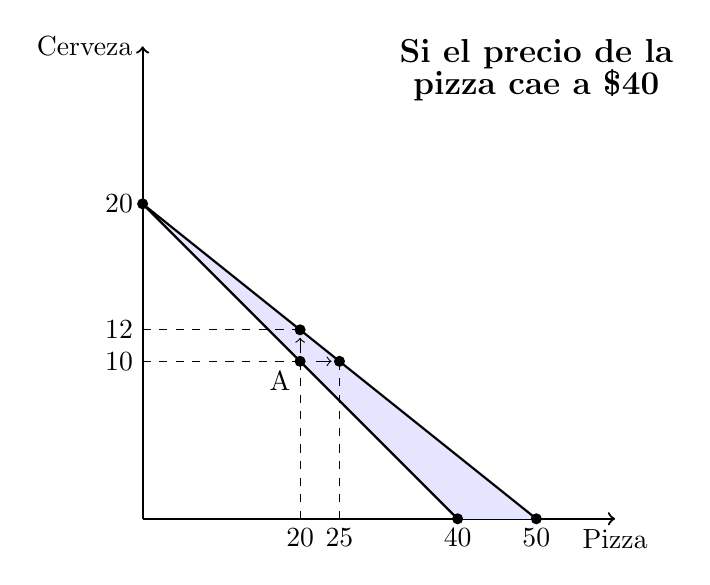
\begin{tikzpicture}
        % Ejes
        \draw[thick,->] (0,0) -- (6,0) node[below] {Pizza};
        \draw[thick,->] (0,0) -- (0,6) node[left] {Cerveza};
    
        % Área sombreada (posibilidades de consumo)
        \fill[blue!10] (0,4) -- (5,0) -- (4,0) -- cycle;
    
        % Líneas de presupuesto (original y desplazada)
        \draw[thick] (0,4) -- (4,0);
        \draw[thick] (0,4) -- (5,0);
    
        % Puntos clave
        \fill (0,4) circle (2pt) node[left] {20};
        \fill (4,0) circle (2pt) node[below] {40};
        \fill (5,0) circle (2pt) node[below] {50};
    
        % Punto A y puntos cercanos
        \fill (2,2) circle (2pt) node[below left] {A};
        \fill (2.5,2) circle (2pt);
        \fill (2,2.4) circle (2pt);
    
        % Líneas punteadas
        \draw[dashed] (2,2) -- (2,0) node[below] {20};
        \draw[dashed] (2,2) -- (0,2) node[left] {10};
        \draw[dashed] (2.5,2) -- (2.5,0) node[below] {25};
        \draw[dashed] (2,2.4) -- (0,2.4) node[left] {12};
    
        % Flechas de desplazamiento
        \draw[->] (2.2,2) -- (2.4,2);
        \draw[->] (2,2.1) -- (2,2.3);
    
        \node at (5,5.9) {\textbf{{\large Si el precio de la}}};
        \node at (5,5.5) {\textbf{{\large pizza cae a \$40}}};
    
    \end{tikzpicture}
    \end{center}
\end{frame}
    
\begin{frame}{El precio de la cerveza}
    \begin{center}
    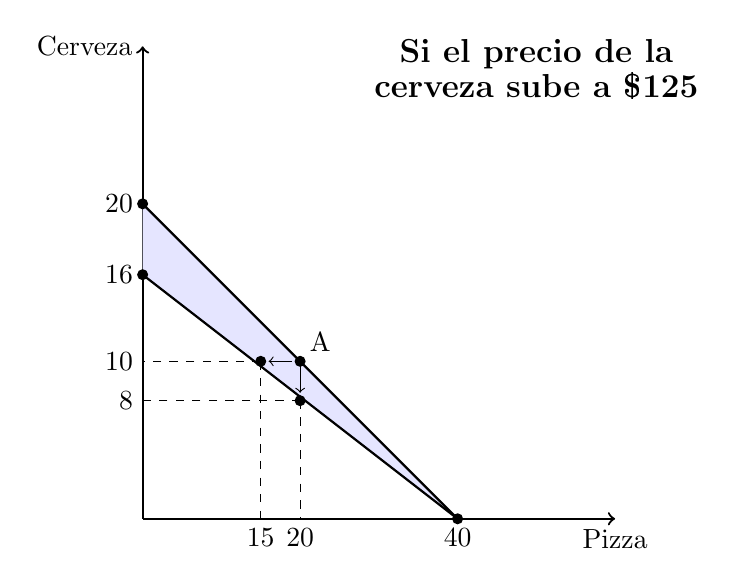
\begin{tikzpicture}
        % Ejes
        \draw[thick,->] (0,0) -- (6,0) node[below] {Pizza};
        \draw[thick,->] (0,0) -- (0,6) node[left] {Cerveza};
    
        % Área sombreada (posibilidades de consumo)
        \fill[blue!10] (0,4) -- (0,3.1) -- (4,0) -- cycle;
    
        % Líneas de presupuesto (original y desplazada)
        \draw[thick] (0,4) -- (4,0);
        \draw[thick] (0,3.1) -- (4,0);
    
        % Puntos clave
        \fill (0,4) circle (2pt) node[left] {20};
        \fill (4,0) circle (2pt) node[below] {40};
        \fill (0,3.1) circle (2pt) node[left] {16};
    
        % Punto A y puntos cercanos
        \fill (2,2) circle (2pt) node[above right] {A};
        \fill (1.5,2) circle (2pt);
        \fill (2,1.5) circle (2pt);
    
        % Líneas punteadas
        \draw[dashed] (2,1.5) -- (2,0) node[below] {20};
        \draw[dashed] (1.5,2) -- (0,2) node[left] {10};
        \draw[dashed] (1.5,2) -- (1.5,0) node[below] {15};
        \draw[dashed] (2,1.5) -- (0,1.5) node[left] {8};
    
        % Flechas de desplazamiento
        \draw[->] (1.9,2) -- (1.6,2);
    
        \draw[->] (2,2) -- (2,1.6);
    
        \node at (5,5.9) {\textbf{{\large Si el precio de la}}};
        \node at (5,5.5) {\textbf{{\large cerveza sube a \$125}}};
    
    \end{tikzpicture}
    \end{center}
\end{frame}
    
    
\begin{frame}{Pendiente}
    \begin{itemize}
        \item Vemos que los cambios en los precios de los bienes modifican la \textbf{inclinación} de la restricción 
        \item La \textbf{pendiente} es la inclinación de una función en un punto particular. Se determina por el cambio vertical con respecto al cambio horizontal. \\ 
         \begin{center}
            $Pendiente =\frac{\Delta Y}{\Delta X} = \frac{\text{Cambio Vertical}}
        {\text{Cambio Horizontal}}$
        \end{center}
        \vspace{1mm}
        \item A lo largo de la restricción presupuestaria gastamos \textbf{todo} el ingreso. Por lo que, sobre la recta, se cumple que lo que dejo de gastar en un bien es igual a lo que comienzo a gastar del otro. 
        \vspace{-7mm}
        \begin{center}
        \[-\Delta Y \times P_Y = \Delta X \times P_X \]
        \end{center}
        \vspace{-4mm}
        Reordenando esa ecuación, obtenemos que:     \vspace{-5mm}
        \begin{center}
        \[\frac{\Delta Y}{\Delta X} = -\frac{P_X}{P_Y} \]
        \end{center}
        Que es lo mismo que la pendiente!
    
    \end{itemize} 
\end{frame}
    
\begin{frame}{Pendiente}
    \begin{itemize}
        \item En el caso de la restricción presupuestaria del ejemplo \\
        \vspace{2mm}
        \begin{center}
            $Pendiente = - \frac{\text{Precio Pizza}}{\text{Precio Cerveza}}= -\frac{P_P}{P_C} = -\frac{50}{100} = -\frac{1}{2}$
        \end{center}
        \vspace{2mm}
        \item Esto nos da una noción de cuánto debo resignar de un bien para poder consumir una unidad más del otro.
        \item En este caso, me dice que para consumir una pizza debo resignar media cerveza. O lo que es lo mismo, el costo de oportunidad de adquirir una porción de pizza adicional es 1/2 cerveza
        \item Vuélvanse fluidos con esto... vean que pueden cambiar los precios de lugar y llego a las mismas conclusiones (pero al revés!).
    \end{itemize}
\end{frame}
    
\begin{frame}{Tasa Marginal de Transformación}
    \begin{itemize}
        \item En el caso de la restricción presupuestaria del ejemplo, este ratio es constante a lo largo de la función, y va a estar dado por los precios relativos de la pizza. \\ \vspace{2mm}
         \begin{center}
        $Pendiente = - \frac{\text{Precio Pizza}}{\text{Precio Cerveza}}= -\frac{P_{Pizza}}{P_{Cerveza}}=-\frac{P_P}{P_C}$
        \end{center}
       \vspace{2mm}
        \item La \textbf{Tasa Marginal de Transformación (TMT)} es la cantidad de un bien que el consumidor debe renunciar para obtener una unidad más del otro bien. Osea, la pendiente!
        \item Viene determinado por los precios de los bienes en el mercado.\\ \vspace{6mm} 
        \begin{center}
          $TMT = - \frac{\text{Precio Pizza}}{\text{Precio Cerveza}}$
          \end{center}
    \end{itemize} 
\end{frame}
    
\begin{frame}{Si rompemos el chanchito o vamos a la casa de la abuela...}
    \begin{center}
    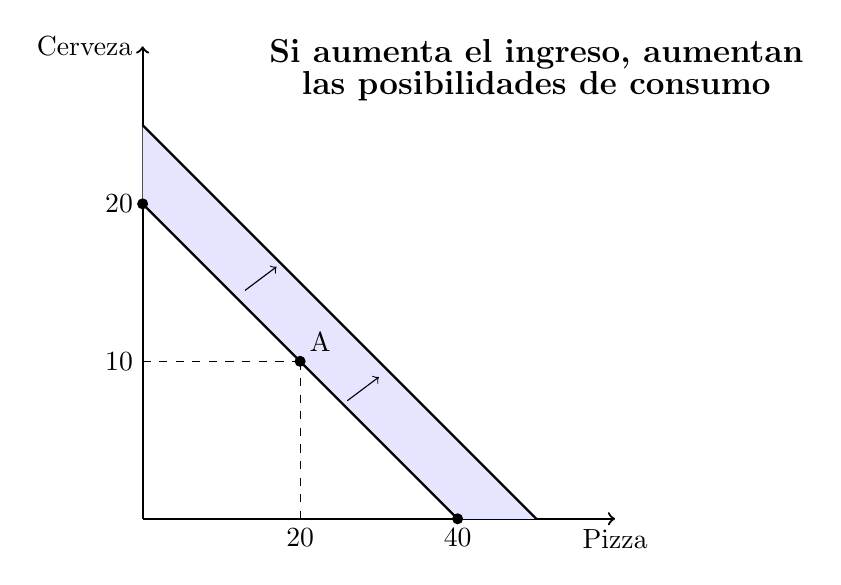
\begin{tikzpicture}
        % Ejes
        \draw[thick,->] (0,0) -- (6,0) node[below] {Pizza};
        \draw[thick,->] (0,0) -- (0,6) node[left] {Cerveza};
    
        % Área sombreada (posibilidades de consumo)
        \fill[blue!10] (0,4) -- (0,5) -- (5,0)-- (4,0) -- cycle;
    
        % Líneas de presupuesto (original y desplazada)
        \draw[thick] (0,4) -- (4,0);
        \draw[thick] (0,5) -- (5,0);
    
        % Puntos clave
        \fill (0,4) circle (2pt) node[left] {20};
        \fill (4,0) circle (2pt) node[below] {40};
    
        % Punto A y puntos cercanos
        \fill (2,2) circle (2pt) node[above right] {A};
    
        % Líneas punteadas
        \draw[dashed] (2,2) -- (2,0) node[below] {20};
        \draw[dashed] (2,2) -- (0,2) node[left] {10};
    
        % Flechas de desplazamiento
        \draw[->] (1.3,2.9) -- (1.7,3.2);
    
        \draw[->] (2.6,1.5) -- (3,1.8);
        (2,2) -- (2,1.6);
    
        \node at (5,5.9) {\textbf{{\large Si aumenta el ingreso, aumentan}}};
        \node at (5,5.5) {\textbf{{\large las posibilidades de consumo}}};
    
    \end{tikzpicture}
    \end{center}
\end{frame}
    
\begin{frame}{Algunos casos especiales}
        \begin{itemize}
        \item En los casos analizados asumimos que el precio del producto no cambia según la cantidad de unidades que adquirimos \vspace{2mm}
        \item En muchos casos no es así...
        \vspace{2mm}
        \begin{itemize}
        \item Precio por cantidad o promoción. \vspace{2mm}
        \item Limite en la cantidad.
        \end{itemize}
        \end{itemize}
\end{frame}
    
\begin{frame}{Promoción en medialunas}
    María solo consume café y medialunas. En la panadería "Luna" venden cada medialuna a \$25, pero si más de 12 salen \$20. El ingreso diario de María es \$500 y el precio de cada café es \$20. 
    
    \begin{center}
    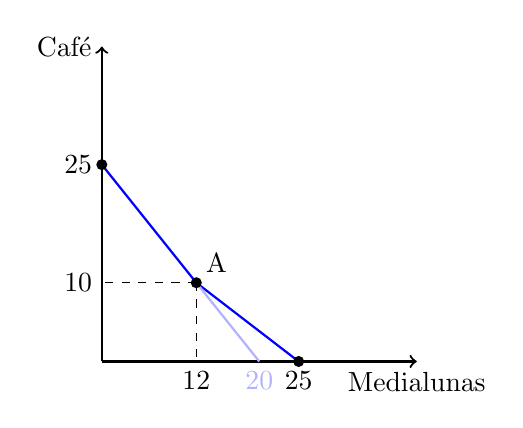
\begin{tikzpicture}
        % Ejes
        \draw[thick,->] (0,0) -- (4,0) node[below ] {Medialunas};
        \draw[thick,->] (0,0) -- (0,4) node[left] {Café};
    
        % RP
        \draw[thick, color=blue] (0,2.5) -- (1.2,1);
        \draw[thick, color=blue] (1.2,1) -- (2.5,0);
        \draw[thick, color=blue!30] (1.2,1) -- (2,0) node[below] {20};
    
        % Puntos clave
        \fill (0,2.5) circle (2pt) node[left] {25};
        \fill (1.2,1) circle (2pt) node[above right] {A};
        \fill (2.5,0) circle (2pt) node[below] {25};
    
        % Línea punteada
        \draw[dashed] (1.2,1) -- (1.2,0) node[below] {12};
        \draw[dashed]  (1.2,1) -- (0,1)  node[left] {10};
        
    \end{tikzpicture}
    \end{center}
\end{frame}
    
\begin{frame}{Límite de consumo de harina}
    Julián dispone de \$2000 para consumir harina y tomate. El kilo de tomate cuesta \$500 y el kilo de harina \$400. Debido a un faltante de harina, solo puede adquirir 2kg por compra. 
    
    \begin{center}
    \begin{tikzpicture}
        % Ejes
        \draw[thick,->] (0,0) -- (7,0) node[below ] {Harina};
        \draw[thick,->] (0,0) -- (0,5) node[left] {Tomate};
    
        % Línea de presupuesto
        \draw[thick, color=blue] (0,4) -- (2,2.4);
        \draw[thick, color=blue] (2,2.4) -- (2,0) node[below] {2};
        \draw[thick, color=blue!30] (2,2.4) -- (5,0) ;
    
        % Puntos clave
        \fill (0,4) circle (2pt) node[left] {4};
        \fill (2,2.4) circle (2pt) node[above right] {A};
        \fill[blue!30] (5,0) circle (2pt) node[below] {5};
    
        % Línea punteada
        \draw[dashed]  (2,2.4) -- (0,2.4)  node[left] {2,4};
    
        \node at (7,3.9) {\includegraphics[width=3.5cm]{../Figures/limite-compra-aceite-harina-3-1024x768.jpg}};
    \end{tikzpicture}
    \end{center}
\end{frame}


\end{document}
